%!TEX root = ../dokumentation.tex

\begin{titlepage}
	\begin{longtable}{p{8cm} p{8cm}}
		{\raisebox{\ht\strutbox-\totalheight}{
\includegraphics[height=2.5cm]{images/cover/logo-dhbw.png}}} &
		{\raisebox{\ht\strutbox-\totalheight}{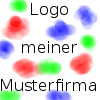
\includegraphics[height=2.5cm]{images/cover/logo-company.png}}}
	\end{longtable}
	\enlargethispage{20mm}
	\begin{center}
    \doublespacing{
		\vspace*{12mm}	{\LARGE\textbf \documentTitle }}\\
		\vspace*{12mm}	{\large\textbf {\documentTypePhrase}}\\
		\vspace*{12mm}	\degreePhrase\\
		\vspace*{3mm}		{\textbf \degree}\\
		\vspace*{12mm}	\departmentPhrase{} \department\\
    \vspace*{0mm}		\locationUniversityPhrase{} \locationUniversity\\
		\vspace*{12mm}	\documentAuthorPhrase\\
		\vspace*{3mm}		{\large\textbf \documentAuthor}\\
		\vspace*{12mm}	\releaseDate\\
	\end{center}
	\vfill
	\begin{spacing}{1.2}
	\begin{tabbing}
		mmmmmmmmmmmmmmmmmmmmmmmmmm             \= \kill
		\textbf{\documentPeriodPhrase}       \>  \documentPeriod\\
		\textbf{\matriculationNumberPhrase, \coursePhrase}  \>  \matriculationNumber, \course\\
		\textbf{\companyPhrase}                  \>  \companyName, \companyLocation\\
		\textbf{\tutorPhrase}               \>  \tutor\\
		\textbf{\evaluatorPhrase}              \>  \evaluator
	\end{tabbing}
	\end{spacing}
\end{titlepage}
